\recipe{Coconut Sweet Potato Soup}
\label{recipe:coconut_sweet_potato_soup}
\makes{Makes enough for two generously}
\worktime{30 minutes}
\totaltime{30 minutes}
\source{From Rachel}

\begin{ingredients}
  \ingroup{Solids}
  \item Udon noodles, 2 packs
  \item Tofu or chicken, \SI{200}{\gram}
  \item Sweet potato, \SI{200}{\gram} cubed
  \item Lotus root, \SI{200}{\gram} sliced
  \item Kale, \SI{200}{\gram} chopped
  \item Garnish: green onions/radishes

  \ingroup{Seasonings}
  \item Garlic, \SI{1}{\tablespoon} crushed
  \item Ginger, \SI{2}{\tablespoon} chopped
  \item Turmeric, \SI{1.5}{\teaspoon}
  \item Green onion, \SI{50}{\gram} sliced
  \item White miso, \SI{1}{\tablespoon}
  \item Rice vinegar, \SI{1}{\tablespoon}
  \item Honey, \SI{1}{\tablespoon}
  \item Mirin, \SI{1}{\tablespoon}
  \item Sriracha/green curry paste, \SI{1}{\tablespoon}

  \ingroup{Liquid}
  \item Water/Stock, \SI{2.5}{\litre}
  \item Coconut milk, \SI{250}{\milli \litre}
\end{ingredients}

\begin{method}
  Microwave potato until tender.

  Fry garlic and ginger in peanut oil for about \SI{30}{\second}. Add turmeric and fry for a further \SI{30}{\second}.

  Add everything else except coconut milk and udon and bring to a boil. 

  Turn off the heat and stir in coconut milk and garnish.
\end{method}



\begin{figure}[h]
  	\centering
  	
  	\begin{tikzpicture}
  		% Save the image in a box to get its dimensions
  		\sbox0{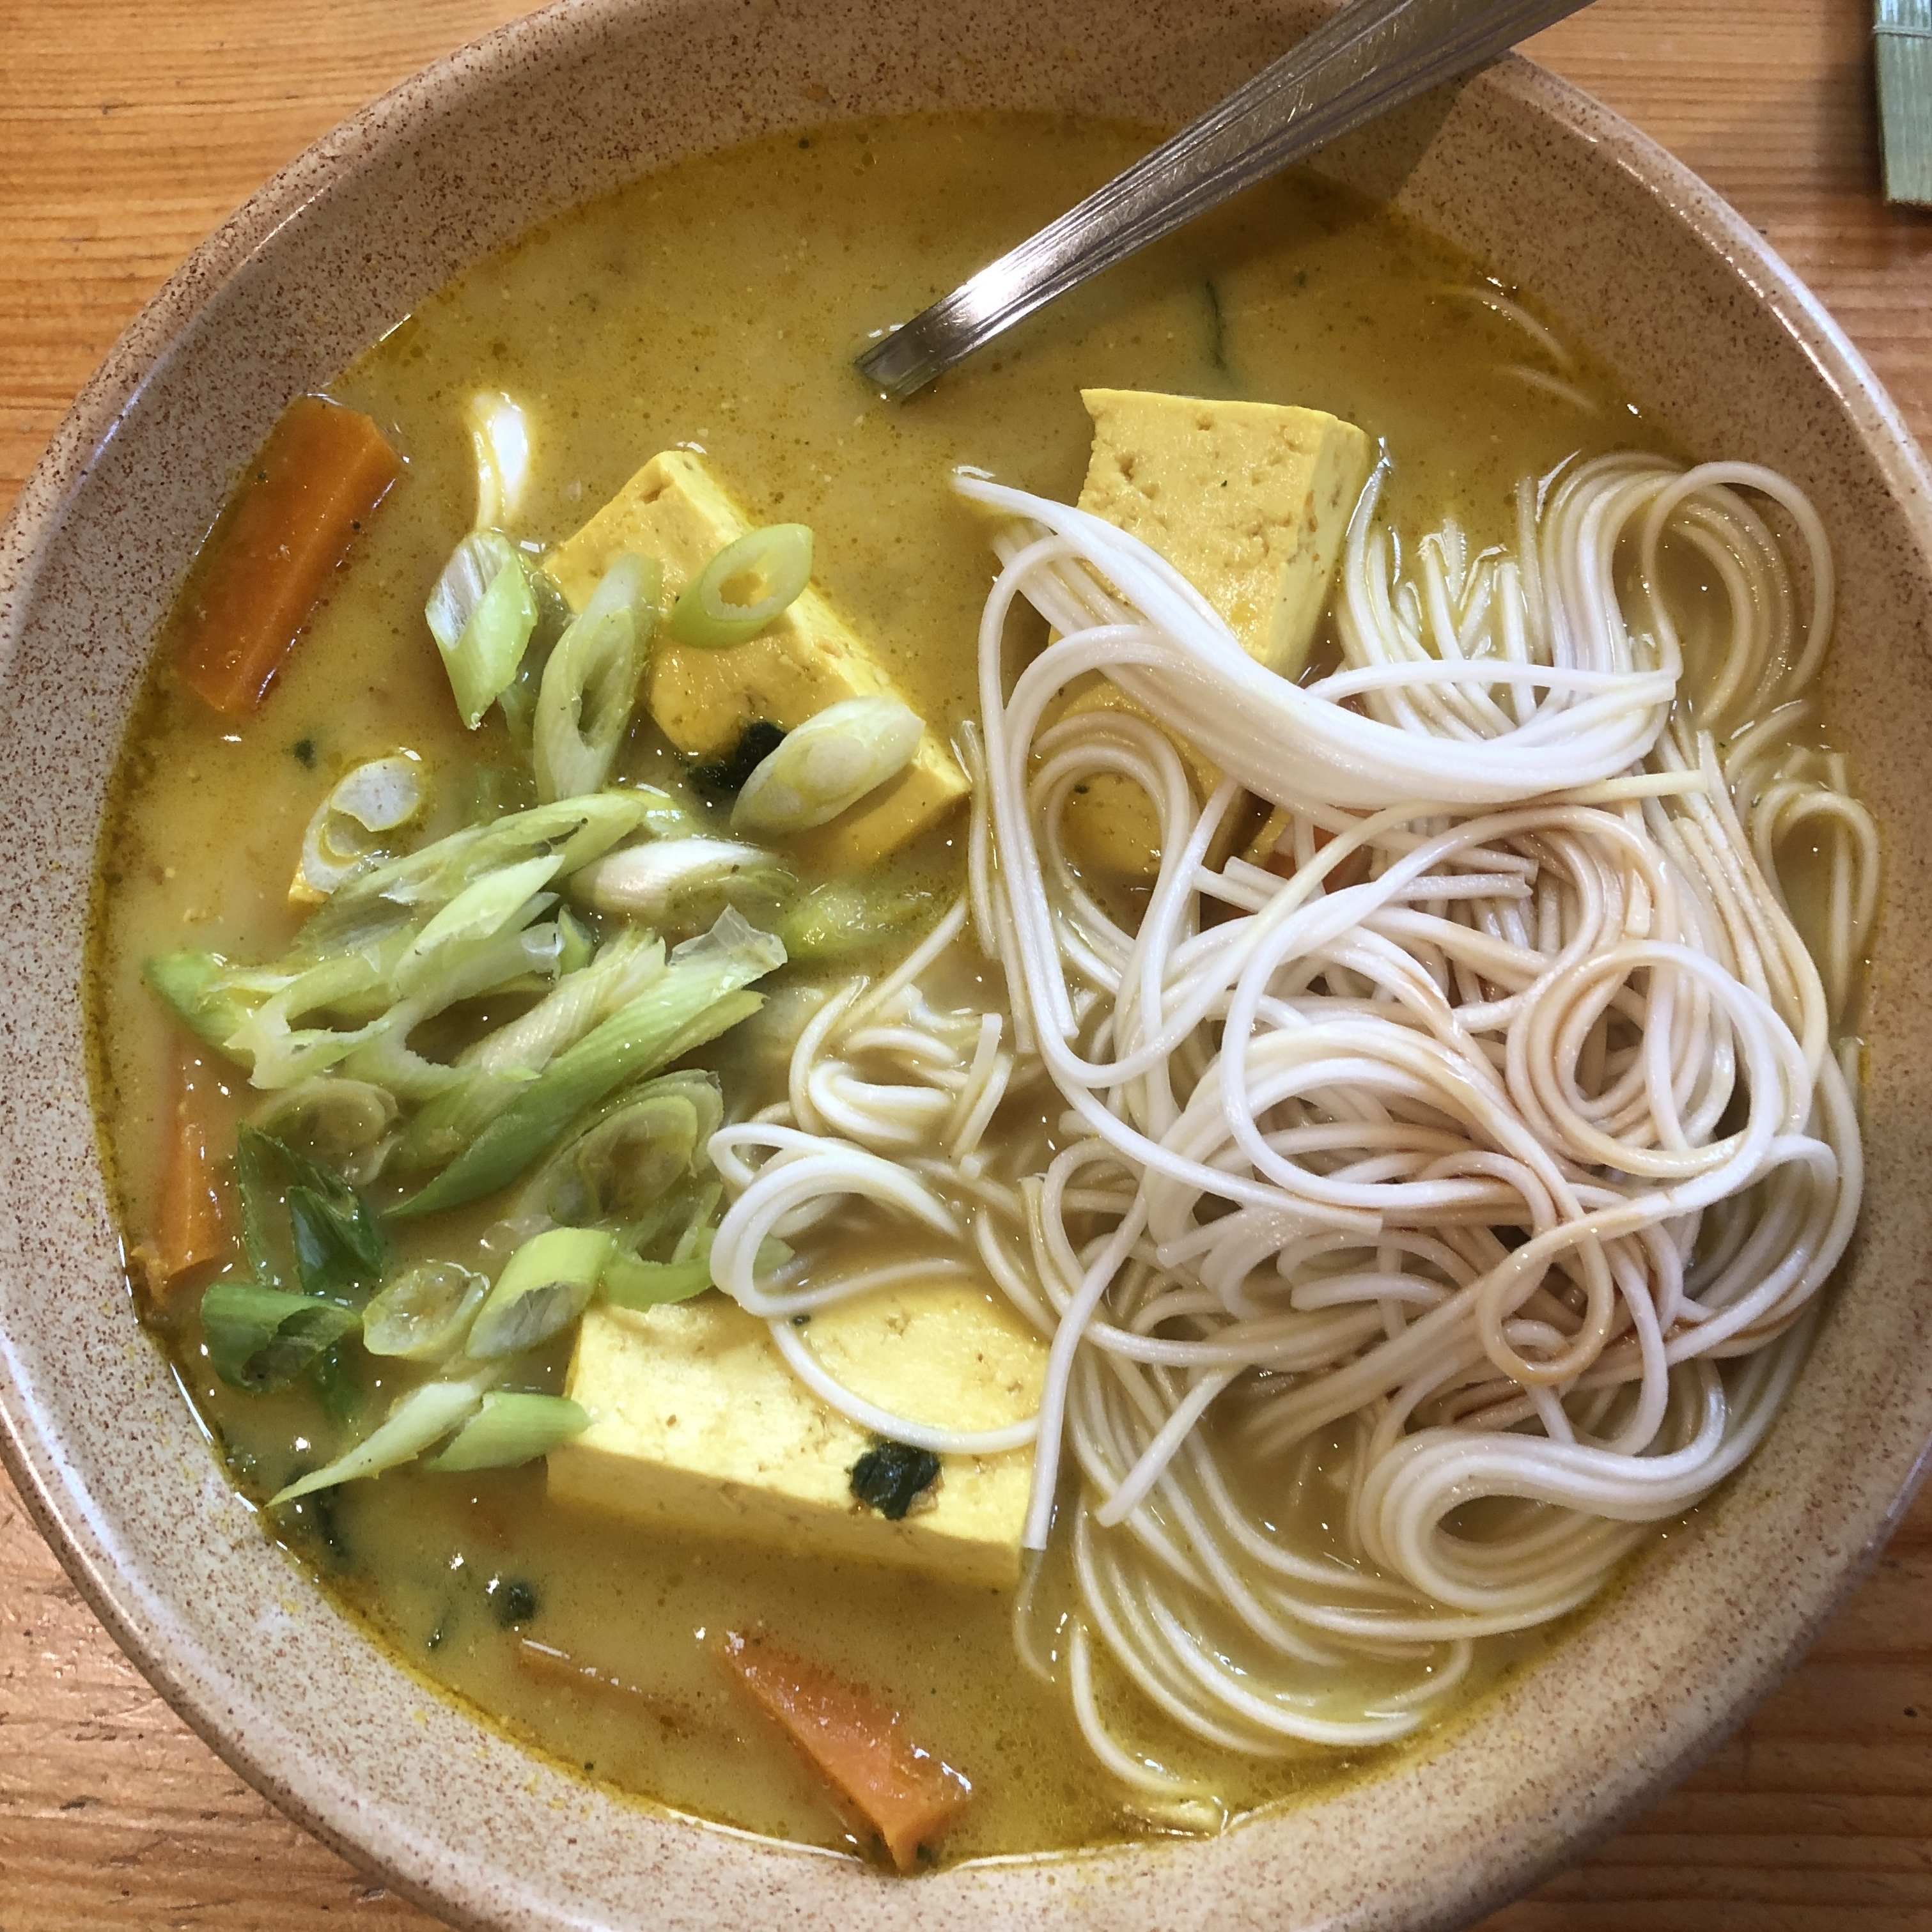
\includegraphics[width = 0.45\linewidth]{images/2023-08-23-soup.jpg}}%
  
  		% Draw a clipping rectangle with rounded corners
  		\path[clip, rounded corners=0.5cm] (0,0) rectangle (\wd0,\ht0);
  
  		% Place the image inside the clipped area
  		\node[inner sep=0pt, outer sep=0pt, anchor=south west] at (0,0) {\usebox0};
	\end{tikzpicture}

  \caption*{}
\end{figure}
